\subsection{Thời gian: Nguyên thủy thời gian – Theo khoảng}
Đồng hồ xoắn ốc (SpiraClock) [98] trực quan hóa thời gian bằng cách sử dụng hình ảnh một chiếc đồng hồ. Hình thức thể hiện bao gồm một mặt đồng hồ và hai kim chỉ giờ và chỉ phút. Mặt trong của đồng hồ hiển thị một hình xoắn ốc kéo dài từ viền của đồng hồ về phía tâm của nó. Mỗi chu kỳ của hình xoắn ốc đại diện cho 12 giờ, với thời gian thực được hiển thị ở chu kỳ ngoài cùng và các mốc thời gian tương lai được hiển thị ở gần trung tâm (trong Hình (\ref{fig:f7.11}) là khoảng 9 tiếng sau trong tương lai). Các khoảng thời gian (ví dụ: các cuộc họp) được thể hiện dưới dạng các phân đoạn được tô màu dọc theo hình xoắn ốc. Các phân đoạn này sẽ thể hiện cho ta biết được thời điểm bắt đầu và kết thúc. Từ đó, người dùng cũng có thể nhanh chóng quan sát được xem liệu các cuộc họp nhất định có bị chồng chéo nhau hay chương trình làm việc có quá dày đặc do nhiều sự kiện liên tiếp nhau hay không. Khi thời gian trôi qua, vòng xoắn ốc được cập nhật liên tục và các khoảng thời gian trong tương lai dần dần di chuyển ra ngoài cho đến khi chúng trở thành thời gian hiện tại (thời gian thực). Song song với đó, các khoảng thời gian quá khứ sẽ dần dần mờ đi. Với cách thức hoạt động như trên, SpiraClock là một phiên bản nâng cấp của chiếc đồng hồ cổ điển khi nó cho phép người dùng xem trước các khoảng thời gian của tương lai gần và đồng thời cũng có thể nắm bắt khái quát về các khoảng thời gian quá khứ. SpiraClock cũng cho phép người dùng di chuyển kim đồng hồ để truy cập tới các thời điểm khác nhau, bên cạnh đó ta cũng có thể đánh dấu để làm nổi bật các khoảng thời gian mà chúng ta quan tâm và tạo ra các ghi chú dạng văn bản kèm theo tương ứng.
\begin{figure}[H] % places figure environment here   
    \centering % Centers Graphic
    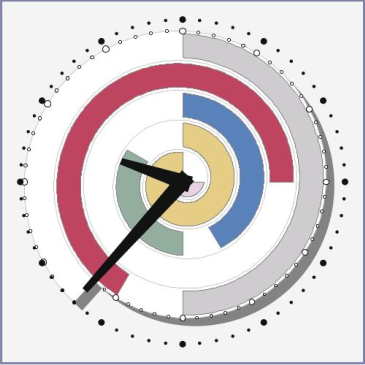
\includegraphics[width=0.8\textwidth]{assets/fig_7_11.png} 
    \caption{SpiraClock [98] được xây dựng dựa trên ý tưởng của màn hình một chiếc đồng hồ. Trong hình, kim phút hiện đang chỉ vào một cuộc họp đang diễn ra. Các cuộc hẹn trong tương lai được xếp dọc theo hình xoắn ốc trên mặt đồng hồ. (Nguồn: Tác giả tổng hợp)} % Creates caption underneath graph
    \label{fig:f7.11}
\end{figure}